%\newpage
\section{Feldman-Cousins throw distributions}\label{sec:fc_appendix}
\begin{figure*}[h]
  \centering
  %\captionsetup[subfloat]{captionskip=-5pt}
  \subfloat[24 kt-MW-yr] {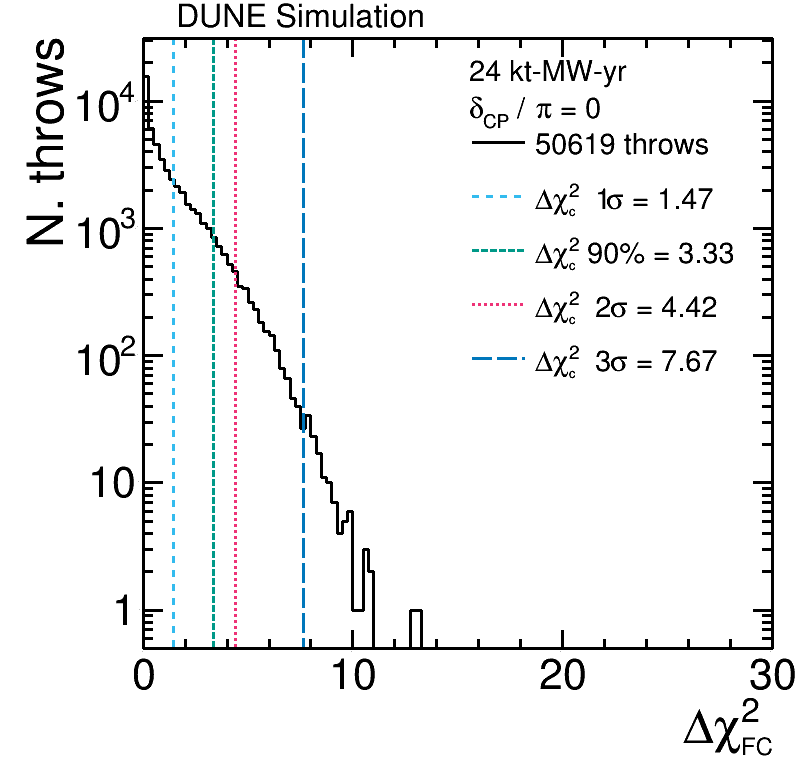
\includegraphics[width=0.33\linewidth]{nh_FC_ndfd_24ktMWyr_dcp0.png}}
  \subfloat[66 kt-MW-yr] {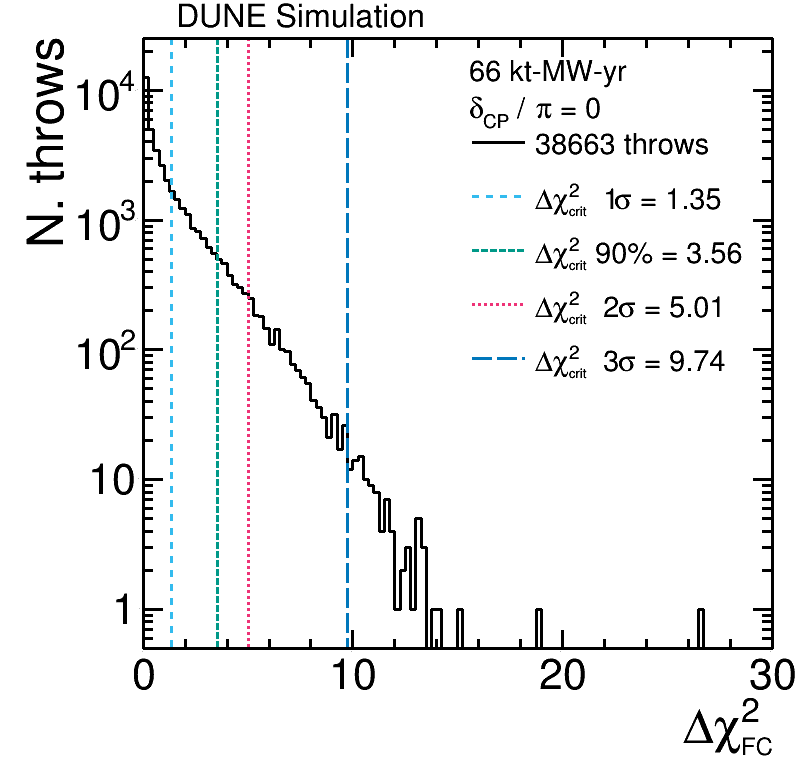
\includegraphics[width=0.33\linewidth]{nh_FC_ndfd_66ktMWyr_dcp0.png}}
  \subfloat[100 kt-MW-yr]{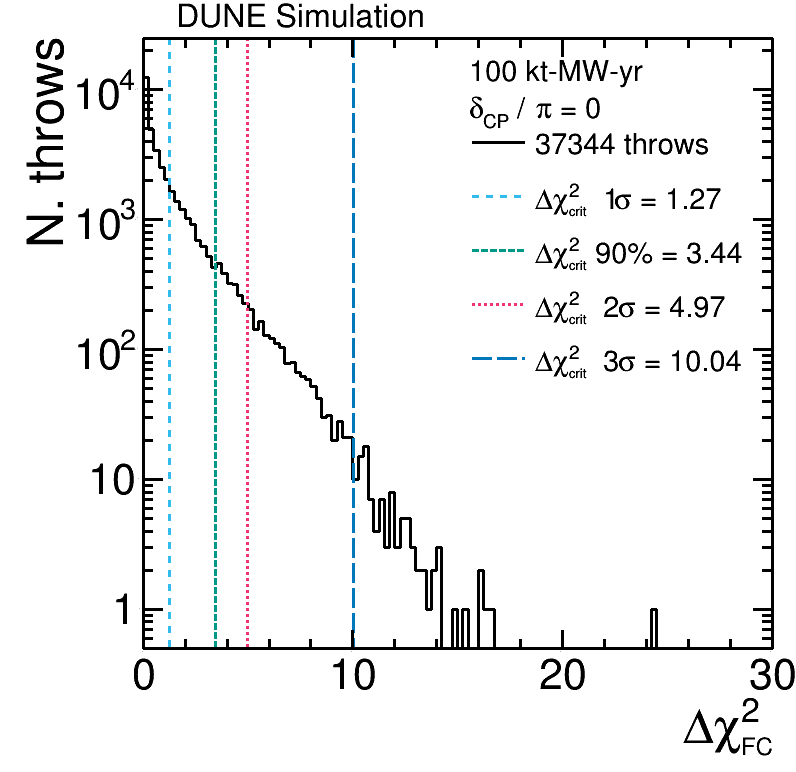
\includegraphics[width=0.33\linewidth]{nh_FC_ndfd_100ktMWyr_dcp0.png}}\\
  \subfloat[150 kt-MW-yr]{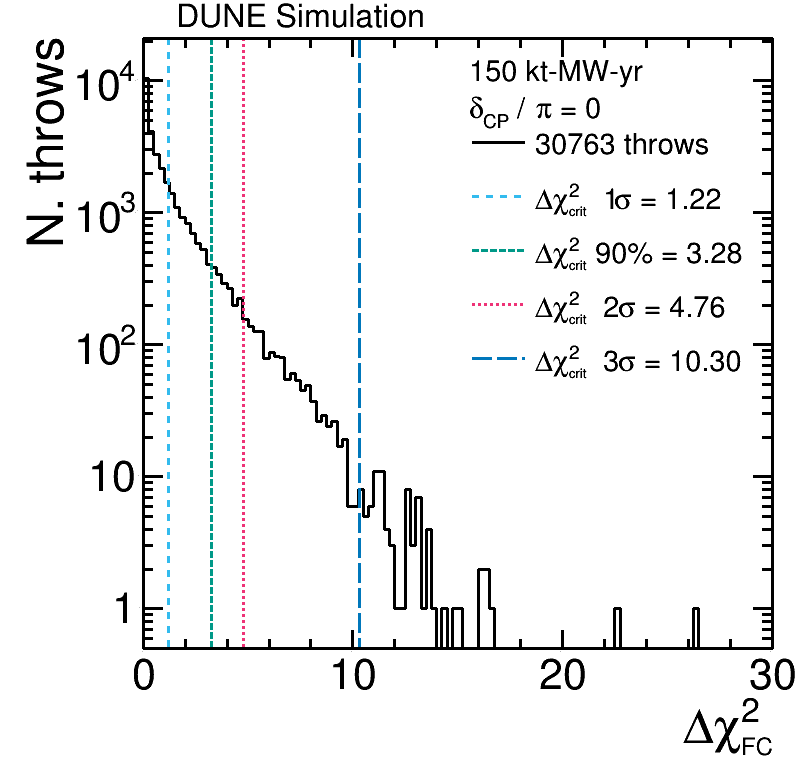
\includegraphics[width=0.33\linewidth]{nh_FC_ndfd_150ktMWyr_dcp0.png}}
  \subfloat[197 kt-MW-yr]{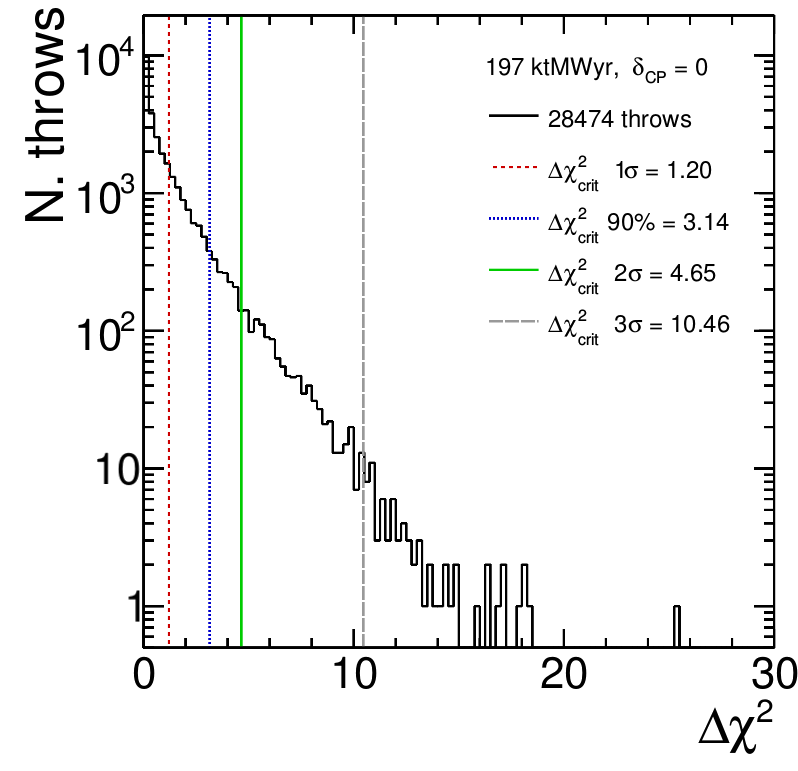
\includegraphics[width=0.33\linewidth]{nh_FC_ndfd_197ktMWyr_dcp0.png}}
  \subfloat[336 kt-MW-yr]{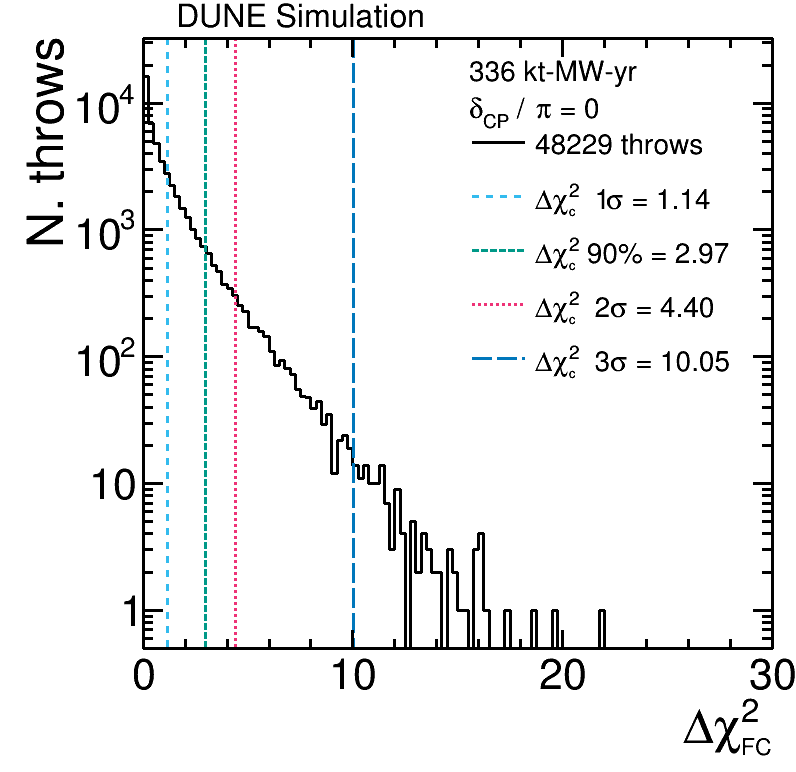
\includegraphics[width=0.33\linewidth]{nh_FC_ndfd_336ktMWyr_dcp0.png}}\\
  \subfloat[500 kt-MW-yr]{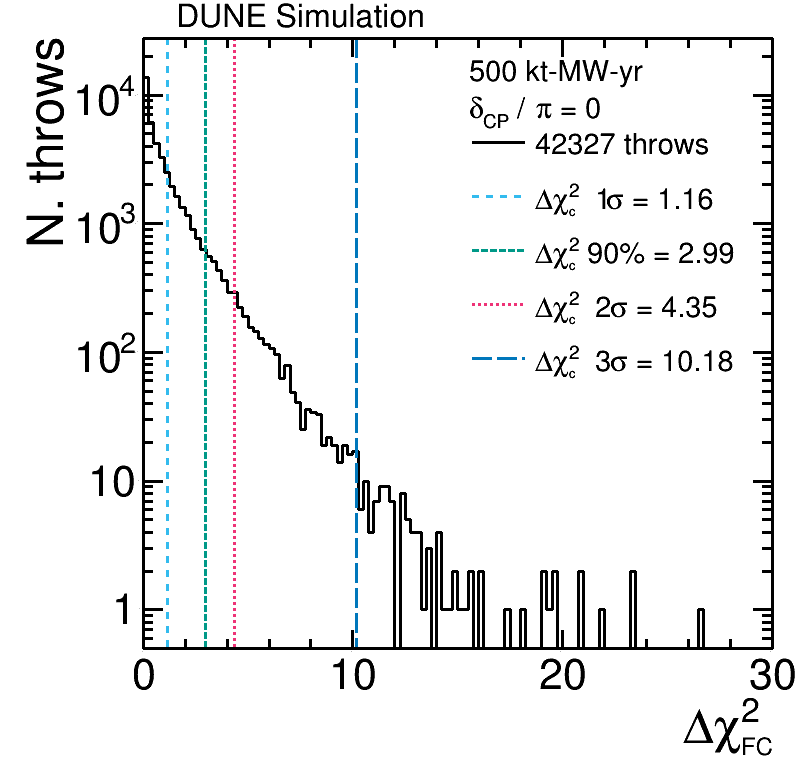
\includegraphics[width=0.33\linewidth]{nh_FC_ndfd_500ktMWyr_dcp0.png}}
  \subfloat[646 kt-MW-yr]{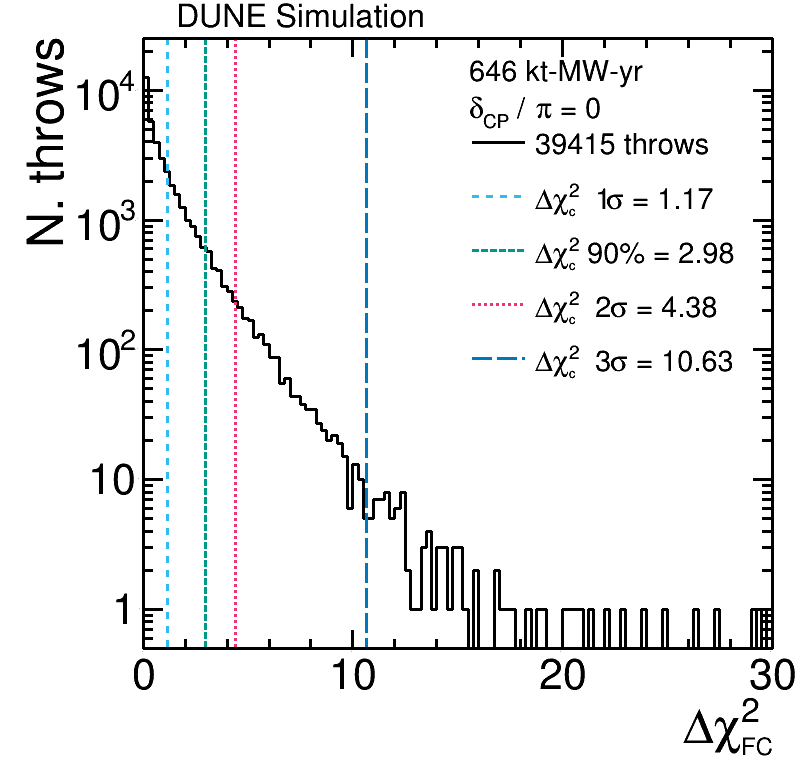
\includegraphics[width=0.33\linewidth]{nh_FC_ndfd_646ktMWyr_dcp0.png}}
  \subfloat[936 kt-MW-yr]{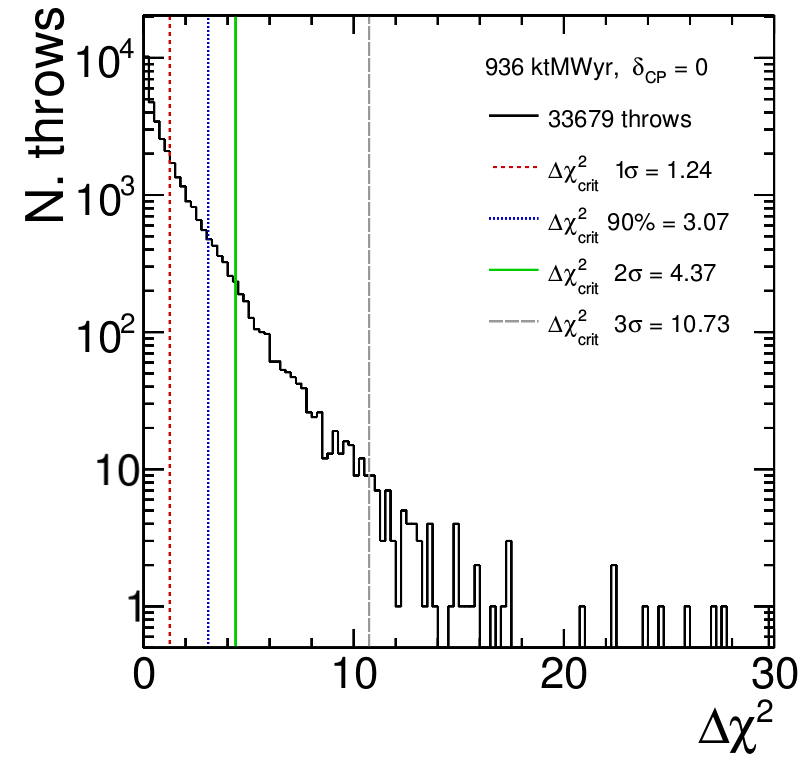
\includegraphics[width=0.33\linewidth]{nh_FC_ndfd_936ktMWyr_dcp0.png}}
  \caption{Distribution of \dchisq values, calculated using Equation~\ref{eq:dchisq_fc}, for a large number of throws with true $\deltacp = 0$, for a variety of exposures. The \dchisqcrit values (vertical lines) obtained using the Feldman-Cousins method show the \dchisqFC value below which 68.27\% (1$\sigma$), 90\%, 95.45\% (2$\sigma$) and 99.73\% (3$\sigma$) of throws reside, with the calculated values given in the legend. The number of throws used is also given. All exposures include an assumption of 57\% accelerator uptime as described in the text.}
  \label{fig:fc_throws_exp}
\end{figure*}
\begin{figure*}[h]
  \centering
  \subfloat[$\deltacp/\pi = -1$]    {\includegraphics[width=0.33\linewidth]{{nh_FC_ndfd_100ktMWyr_dcp-1}.png}}
  \subfloat[$\deltacp/\pi = -0.75$] {\includegraphics[width=0.33\linewidth]{{nh_FC_ndfd_100ktMWyr_dcp-0.75}.png}}
  \subfloat[$\deltacp/\pi = -0.5$]  {\includegraphics[width=0.33\linewidth]{{nh_FC_ndfd_100ktMWyr_dcp-0.5}.png}}\\
  \subfloat[$\deltacp/\pi = -0.25$] {\includegraphics[width=0.33\linewidth]{{nh_FC_ndfd_100ktMWyr_dcp-0.25}.png}}
  \subfloat[$\deltacp/\pi = 0$]     {\includegraphics[width=0.33\linewidth]{{nh_FC_ndfd_100ktMWyr_dcp0}.png}}
  \subfloat[$\deltacp/\pi = 0.25$]  {\includegraphics[width=0.33\linewidth]{{nh_FC_ndfd_100ktMWyr_dcp0.25}.png}}\\
  \subfloat[$\deltacp/\pi = 0.5$]   {\includegraphics[width=0.33\linewidth]{{nh_FC_ndfd_100ktMWyr_dcp0.5}.png}}
  \subfloat[$\deltacp/\pi = 0.75$]  {\includegraphics[width=0.33\linewidth]{{nh_FC_ndfd_100ktMWyr_dcp0.75}.png}}
  \subfloat[$\deltacp/\pi = 1$]     {\includegraphics[width=0.33\linewidth]{{nh_FC_ndfd_100ktMWyr_dcp1}.png}}
  \caption{Distribution of \dchisq values, calculated using Equation~\ref{eq:dchisq_fc}, for a large number of throws for 9 different values of true \deltacp, for a 100 kt-MW-yr exposure. The \dchisqcrit values (vertical lines) obtained using the Feldman-Cousins method show the \dchisqFC value below which 68.27\% (1$\sigma$), 90\%, 95.45\% (2$\sigma$) and 99.73\% (3$\sigma$) of throws reside, with the calculated values given in the legend. The number of throws used is also given. All exposures include an assumption of 57\% accelerator uptime as described in the text.}
  \label{fig:fc_throws_100kt-MW-yr}
\end{figure*}
\begin{figure*}[h]
  \centering
  \subfloat[$\deltacp/\pi = -1$]    {\includegraphics[width=0.33\linewidth]{{nh_FC_ndfd_336ktMWyr_dcp-1}.png}}
  \subfloat[$\deltacp/\pi = -0.75$] {\includegraphics[width=0.33\linewidth]{{nh_FC_ndfd_336ktMWyr_dcp-0.75}.png}}
  \subfloat[$\deltacp/\pi = -0.5$]  {\includegraphics[width=0.33\linewidth]{{nh_FC_ndfd_336ktMWyr_dcp-0.5}.png}}\\
  \subfloat[$\deltacp/\pi = -0.25$] {\includegraphics[width=0.33\linewidth]{{nh_FC_ndfd_336ktMWyr_dcp-0.25}.png}}
  \subfloat[$\deltacp/\pi = 0$]     {\includegraphics[width=0.33\linewidth]{{nh_FC_ndfd_336ktMWyr_dcp0}.png}}
  \subfloat[$\deltacp/\pi = 0.25$]  {\includegraphics[width=0.33\linewidth]{{nh_FC_ndfd_336ktMWyr_dcp0.25}.png}}\\
  \subfloat[$\deltacp/\pi = 0.5$]   {\includegraphics[width=0.33\linewidth]{{nh_FC_ndfd_336ktMWyr_dcp0.5}.png}}
  \subfloat[$\deltacp/\pi = 0.75$]  {\includegraphics[width=0.33\linewidth]{{nh_FC_ndfd_336ktMWyr_dcp0.75}.png}}
  \subfloat[$\deltacp/\pi = 1$]     {\includegraphics[width=0.33\linewidth]{{nh_FC_ndfd_336ktMWyr_dcp1}.png}}
  \caption{Distribution of \dchisq values, calculated using Equation~\ref{eq:dchisq_fc}, for a large number of throws for 9 different values of true \deltacp, for a 336 kt-MW-yr exposure. The \dchisqcrit values (vertical lines) obtained using the Feldman-Cousins method show the \dchisqFC value below which 68.27\% (1$\sigma$), 90\%, 95.45\% (2$\sigma$) and 99.73\% (3$\sigma$) of throws reside, with the calculated values given in the legend. The number of throws used is also given. All exposures include an assumption of 57\% accelerator uptime as described in the text.}
  \label{fig:fc_throws_336kt-MW-yr}
\end{figure*}
The distribution of throws used to calculate the \dchisqcrit values for Figure~\ref{fig:fc_vs_exp} for nine different exposures with $\deltacp = 0$ are shown in Figure~\ref{fig:fc_throws_exp}; for Figure~\ref{fig:fc_vs_dcp_100} for nine different values of \deltacp with an exposure of 100 kt-MW-yr in Figure~\ref{fig:fc_throws_100kt-MW-yr}; and for Figure~\ref{fig:fc_vs_dcp_336} for nine different values of \deltacp with an exposure of 336 kt-MW-yr in Figure~\ref{fig:fc_throws_336kt-MW-yr}. For each distribution shown in Figures~\ref{fig:fc_throws_exp},~\ref{fig:fc_throws_100kt-MW-yr} and~\ref{fig:fc_throws_336kt-MW-yr}, the calculated \dchisqcrit values corresponding to for 68.27\% (1$\sigma$), 90\%, 95.45\% (2$\sigma$) and 99.73\% (3$\sigma$) of the throws are given and indicated with a vertical line. The number of throws used is also given. The \dchisqcrit values were only calculated up to the 3$\sigma$ level due to the very large number of throws required for higher confidence levels.
